\section{Mechanical Turk}
	Many references taken from \url{http://homepage.psy.utexas.edu/homepage/faculty/gosling/reprints/MTurkhowto.pdf}
	\subsection{Survey}
		\url{https://docs.google.com/forms/d/1UyG0kVirpdmQ-1C3Qq9aMKM9ROu0gJV0b40mjtYz4uo/viewform} \\
		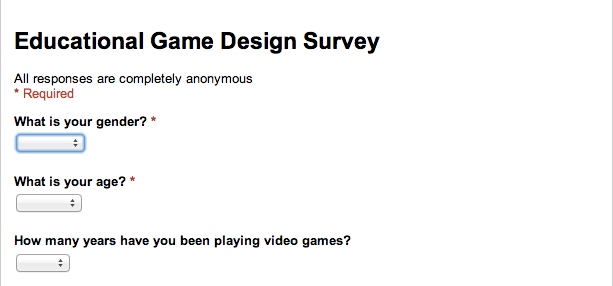
\includegraphics[width = \textwidth]{img/survey1.png}
		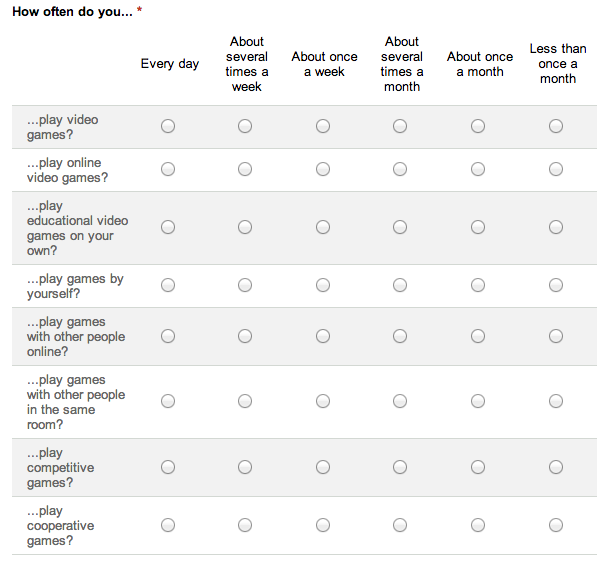
\includegraphics[width = \textwidth]{img/survey2.png}
		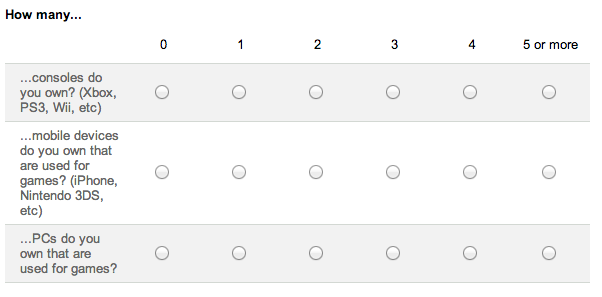
\includegraphics[width = \textwidth]{img/survey3.png}
		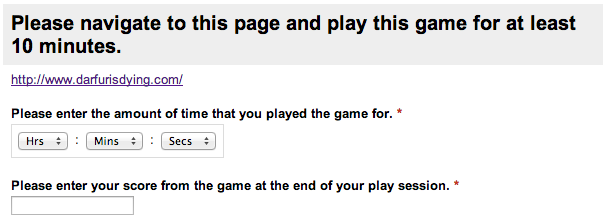
\includegraphics[width = \textwidth]{img/survey4.png}
		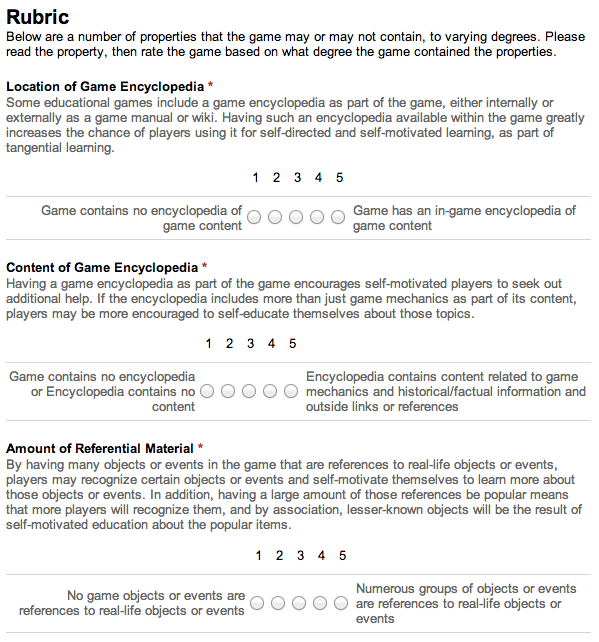
\includegraphics[width = \textwidth]{img/survey5.png}
		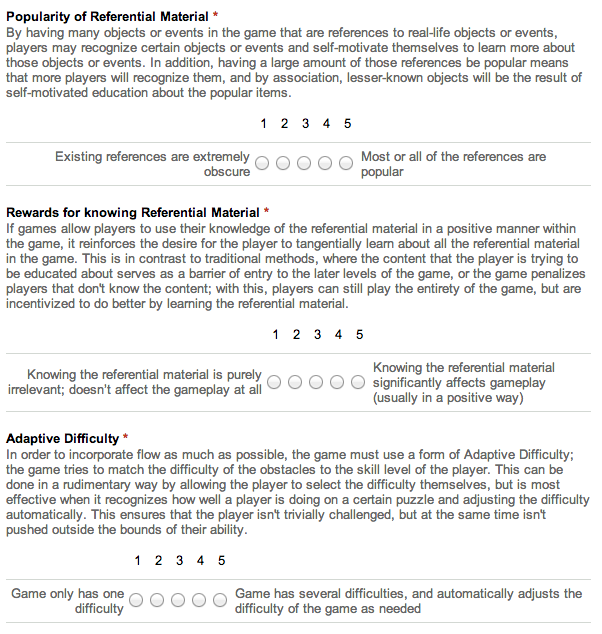
\includegraphics[width = \textwidth]{img/survey6.png}
		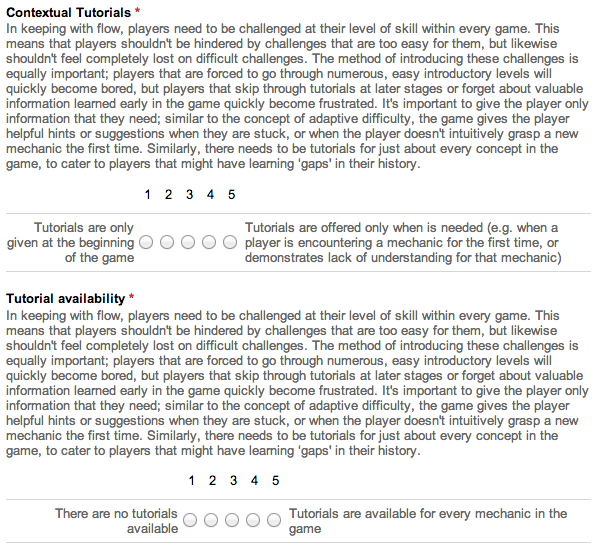
\includegraphics[width = \textwidth]{img/survey7.png}
		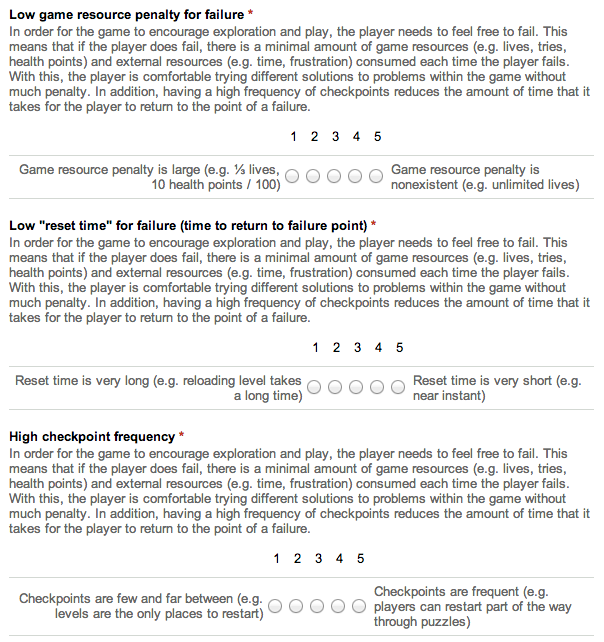
\includegraphics[width = \textwidth]{img/survey8.png}
		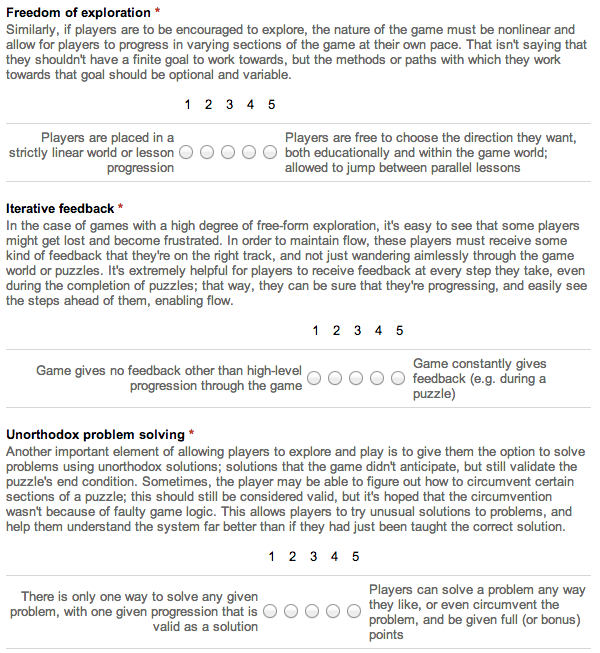
\includegraphics[width = \textwidth]{img/survey9.png}
		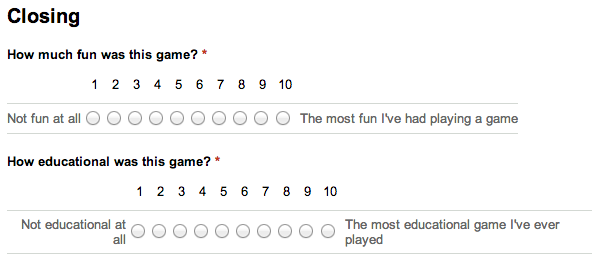
\includegraphics[width = \textwidth]{img/survey10.png}
		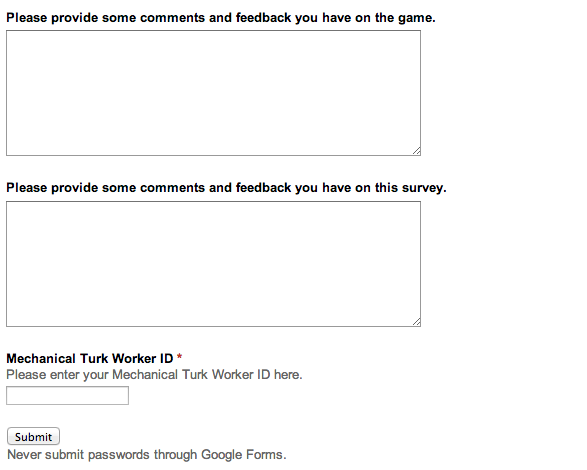
\includegraphics[width = \textwidth]{img/survey11.png}
	\subsection{Survey Design}
		% \subsubsection{Gamer Demographic Information}
	\subsection{Compensation Scheme}
		Mechanical Turk workers are commonly compensated at 10 cents per person per 10 minute response. This seems more than adequate; however, the rate will begin at \$0.05 per survey response. If the requisite number of responses hasn't been received in one week, the rate will increase to \$0.10 per survey response, and will continue to increase each \$0.05 each week until all the survey responses are received.
	\subsection{Ensuring High-Quality Responses}
		To ensure high-quality survey responses, there are a number of measures that can be taken. The first is the criteria option built in to Mechanical Turk for workers. It's recommended to avoid translation issues by restricting to US workers only, and to filter out workers with a bad history of responses by using a 95\% HIT acceptance rate criteria.

		It is harder to ensure that the workers actually play the requisite amount of the game. To combat workers not actually playing the game, the workers will be required to upload a screenshot of their final score playing the game. This screenshot can be searched for online to see if they uploaded an image found elsewhere; if so, the result will be rejected.

		The hardest part will be to ensure that the workers fill the form out without providing any bogus responses. There's not much that can be done for this (due to us testing to see if the rubric is excessively vague), but we can implement safegaurds such as the cleverly-hidden "answer this number for this question" section.